\documentclass[a4paper,UTF8]{article}
\usepackage{ctex}
\usepackage[margin=1.25in]{geometry}
\usepackage{color}
\usepackage{graphicx}
\usepackage{amssymb}
\usepackage{amsmath}
\usepackage{amsthm}
\usepackage{enumerate}
\usepackage{bm}
\usepackage{hyperref}
\usepackage{epsfig}
\usepackage{color}
\usepackage{booktabs}
\usepackage{tcolorbox}
\usepackage{mdframed}
\usepackage{lipsum}
\newmdtheoremenv{thm-box}{myThm}
\newmdtheoremenv{prop-box}{Proposition}
\newmdtheoremenv{def-box}{定义}

\setlength{\evensidemargin}{.25in}
\setlength{\textwidth}{6in}
\setlength{\topmargin}{-0.5in}
\setlength{\topmargin}{-0.5in}
% \setlength{\textheight}{9.5in}
%%%%%%%%%%%%%%%%%%此处用于设置页眉页脚%%%%%%%%%%%%%%%%%%
\usepackage{fancyhdr}
\usepackage{lastpage}
\usepackage{layout}
\footskip = 10pt
\pagestyle{fancy}                    % 设置页眉
\lhead{2022年秋季}
\chead{时间序列分析}
% \rhead{第\thepage/\pageref{LastPage}页}
\rhead{作业一}
\cfoot{\thepage}
\renewcommand{\headrulewidth}{1pt}  			%页眉线宽,设为0可以去页眉线
\setlength{\skip\footins}{0.5cm}    			%脚注与正文的距离
\renewcommand{\footrulewidth}{0pt}  			%页脚线宽,设为0可以去页脚线

\makeatletter 									%设置双线页眉
\def\headrule{{\if@fancyplain\let\headrulewidth\plainheadrulewidth\fi%
\hrule\@height 1.0pt \@width\headwidth\vskip1pt	%上面线为1pt粗
\hrule\@height 0.5pt\@width\headwidth  			%下面0.5pt粗
\vskip-2\headrulewidth\vskip-1pt}      			%两条线的距离1pt
 \vspace{6mm}}     								%双线与下面正文之间的垂直间距
\makeatother

%%%%%%%%%%%%%%%%%%%%%%%%%%%%%%%%%%%%%%%%%%%%%%
\numberwithin{equation}{section}
%\usepackage[thmmarks, amsmath, thref]{ntheorem}
\newtheorem{myThm}{myThm}
\newtheorem*{myDef}{Definition}
\newtheorem*{mySol}{Solution}
\newtheorem*{myProof}{Proof}
\newcommand{\indep}{\rotatebox[origin=c]{90}{$\models$}}
\newcommand*\diff{\mathop{}\!\mathrm{d}}

\usepackage{multirow}

%--

%--
\begin{document}
\title{时间序列分析\\
作业一}
\author{191220129, 邢尚禹, starreeze@foxmail.com}
\maketitle

\section*{作业提交注意事项}
\begin{tcolorbox}
\begin{enumerate}
  \item[(1)] 请严格参照教学立方网站所述提交作业,压缩包命名统一为{\color{red}学号\_姓名.zip};
  \item[(2)] 未按照要求提交作业,或提交作业格式不正确,将会被扣除部分作业分数;
  \item[(3)] 除非有特殊情况(如因病缓交),否则截止时间后不接收作业,本次作业记零分。
\end{enumerate}
\end{tcolorbox}

\section{[100pts] 预处理、简单模型和评价指标}
\href{https://github.com/zhouhaoyi/ETDataset}{ETT (Electricity Transformer Temperature)数据集}是一个多变量时间序列数据集,本次实验选取ETTh1中``油温(OT)"组分作为单独的单变量时间序列,该序列记录了每个小时(h)的油温变化,学生需要以此序列为实验对象,实现若干预处理方法、简单模型和评价指标。数据集、代码分别保存在data、code文件夹下。学生需要完成的任务如下:
\begin{enumerate}[ {(}1{)}]
\item 在transforms.py中实现归一化(normalization), 标准化(Standardization),平均归一化(Mean Normalization),Box-Cox变换,需继承Transform类并实现其抽象方法;
\item 在models.py中实现$Naive_1$,$Naive_s$(以24h为周期),Drift模型,需继承ForecastModel类并实现其抽象方法;
\item 在metrics.py中实现MSE,MAE,MAPE,sMAPE,	MASE。
\item 修改并运行main.py,汇报(2)中不同方法,在(1)中不同变换下,用(3)中不同指标衡量的性能,以表格形式呈现,表格示例如表\ref{tb:example}所示。绘制并报告(2)中模型真实序列与预测序列的曲线图(变换方式任选,但需在解答中说明)。
\end{enumerate}
注:utils.py中包含了一些有用的函数,请勿对其进行修改,如有疑问可联系助教。最终需提交的文件为: 1. 修改后的代码,\underline{要求附加一个markdown格式的文件README.md},说明如何复现报告中的结果。2. pdf形式的报告,报告需\textit{描述各个功能的实现(例如以数学公式的形式)}并报告结果,写于\textbf{solution}部分即可。
\begin{mySol}
~\\
\textbf{1. Tramsform}

由于要实现逆变换,必须要在变换时存储训练数据中相关的量,例如Normalization需要存min,max。在做逆变换时,使用这些存储的量作为变换的参数。
下面简述各个变换涉及的数学公式。具体的代码实现很简单,不再赘述。 \\
Normalization:
$$
y_t'=\frac{y_t-y_{min}}{y_{max}-y(min)}
$$
Standardization:
$$
y_t'=\frac{y_t-\mu}{\sigma}
$$
Mean Normalization:
$$
y_t'=\frac{y_t-\mu}{y_{max}-y_{min}}
$$
BoxCox (负值修正):
$$
y_t^{(\lambda)}=\frac{(y_t+\lambda_2)^{\lambda_1}-1}{\lambda_1}, \lambda_1 \neq 0
$$
根据数据,这里取$\lambda_2=0.5$。
\\
\\
\textbf{2. Forcast Model}

各个模型在fit时直接存储整个序列,predict时根据存储的序列来预测。

Naive1直接取最后一个值即可。

NaiveS根据ppt上的公式计算,但在写代码时需要注意ppt上的公式是1-index的,而代码中需要0-index。因此,最终要使用的式子是这样的:

Y[h] = X[n + h - m * (h // m + 1)].

Drift也要注意下标,处理时比NaiveS简单一点:

Y[h] = X[-1] + h * (X[-1] - X[0]) / (len(X) - 1)
\\
\\
\textbf{3. Metric}

代码实现较为简单,这里仅简述数学公式。
\\
MAE:
$$
\frac{1}{H}\sum_{i=1}^{H}|y_{n+i}-y'_{n+i}|
$$
MSE:
$$
\frac{1}{H}\sum_{i=1}^{H}(y_{n+i}-y'_{n+i})^2
$$
MAPE:
$$
\frac{100}{H}\sum_{i=1}^{H}\frac{|y_{n+i}-y'_{n+i}|}{|y_{n+i}|}
$$
注意到这里分母可能为0,代码实现时直接舍弃小于1e-3的项。
\\
SMAPE:
$$
\frac{200}{H}\sum_{i=1}^{H}\frac{|y_{n+i}-y'_{n+i}|}{|y_{n+i}|+|y'_{n+i}|}
$$
MASE:
$$
\frac{(N+H-m)\sum_{i=1}^{H}|y_{n+i}-y'_{n+i}|}{H\sum_{j=m+1}^{N+H}|y_j-y_{j-m}|}
$$

\begin{table}[]
	\centering
	\caption{结果}
	\begin{tabular}{ccccccc}
		\toprule
		Model                      & Transform & MSE & MAE & MAPE & sMAPE & MASE \\
		\midrule
		\multirow{5}{*}{$Naive_1$}
		& None      & 18.66 & 3.535 & 111.8 & 53.58 & 1.649 \\
		& Normalize  & 18.66 & 3.535 & 111.8 & 53.58 & 1.649 \\
		& Standardize & 18.66 & 3.535 & 111.8 & 53.58 & 1.649  \\
		& Mean Normalize & 18.66 & 3.535 & 111.8 & 53.58 & 1.649 \\
		& Box-Cox ($\lambda=0.5$)  & 18.66 & 3.535 & 111.8 & 53.58 & 1.649 \\
		\midrule
		\multirow{5}{*}{$Naive_S$}
		& None      & 28.80 & 4.400 & 138.7 & 59.92 & 2.052 \\
		& Normalize  & 28.80 & 4.400 & 138.7 & 59.92 & 2.052 \\
		& Standardze & 28.80 & 4.400 & 138.7 & 59.92 & 2.052 \\
		& Mean Normalize & 28.80 & 4.400 & 138.7 & 59.92 & 2.052 \\
		& Box-Cox ($\lambda=0.5$) & 28.80 & 4.400 & 138.7 & 59.92 & 2.052 \\
		\midrule
		\multirow{5}{*}{Drift}
		& None      & 42.37 & 5.030 & 85.44 & 99.98 & 2.346 \\
		& Normalize  & 42.37 & 5.030 & 85.44 & 99.98 & 2.346 \\
		& Standardze & 42.37 & 5.030 & 85.44 & 99.98 & 2.346 \\
		& Mean Normalize & 42.37 & 5.030 & 85.44 & 99.98 & 2.346 \\
		& Box-Cox ($\lambda=0.5$) & 22.19 & 3.889 & 84.64 & 66.28 & 1.814 \\
		\bottomrule
	\end{tabular}
\label{tb:result}
\end{table}
~\\
绘制的预测图像如下:
\begin{figure}[htbp]
	\centering
	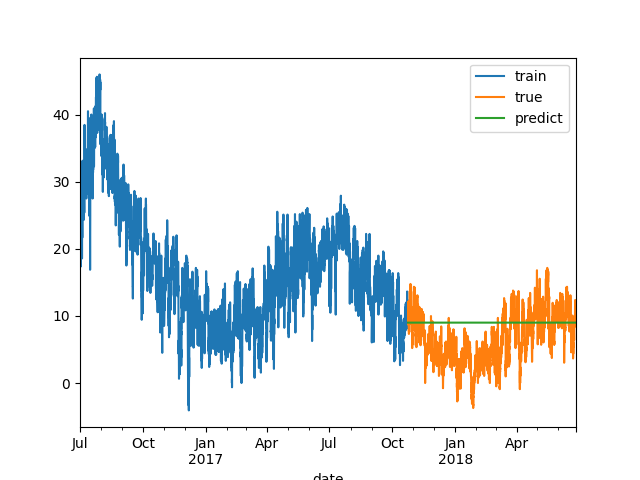
\includegraphics[width=0.85\textwidth]{1}
	\caption{Naive1}
\end{figure}
\begin{figure}[htbp]
	\centering
	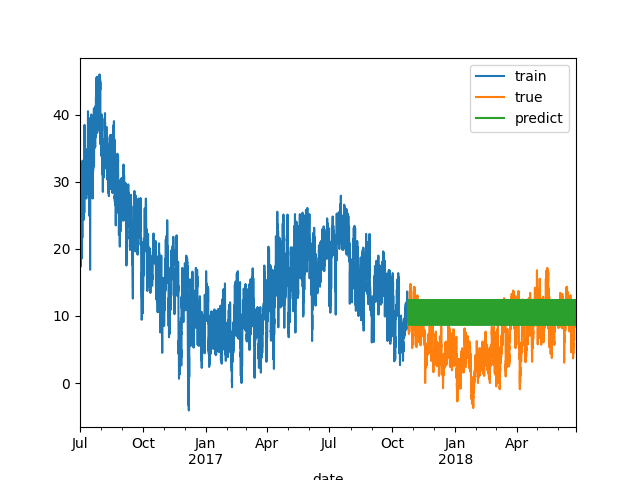
\includegraphics[width=0.85\textwidth]{2}
	\caption{NaiveS}
\end{figure}
\begin{figure}[htbp]
	\centering
	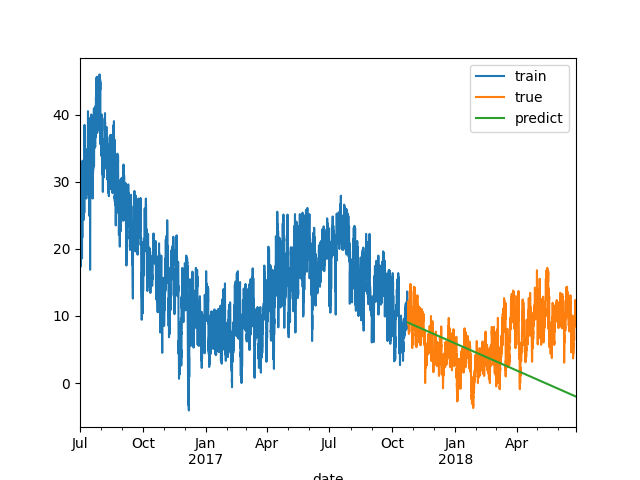
\includegraphics[width=0.85\textwidth]{3}
	\caption{Drift}
\end{figure}

\end{mySol}

\newpage
\section{[附加题20pts] 周期的影响}
在上一题中,我们指定了$Naive_s$方法中的周期为天(24h),本题中学生需要尝试使用不同的周期,考察不同周期下$Naive_s$模型的性能变化。请绘制出模型性能随不同周期的变化曲线。在ETTh1的OT序列上,最好的周期是什么?你可以得出什么结论?
\begin{mySol}
~\\
为了研究周期对性能的影响,设置步长为12h,步数为100,分别对每一步预测并计算mse。结果如下图:
\begin{figure}[htbp]
	\centering
	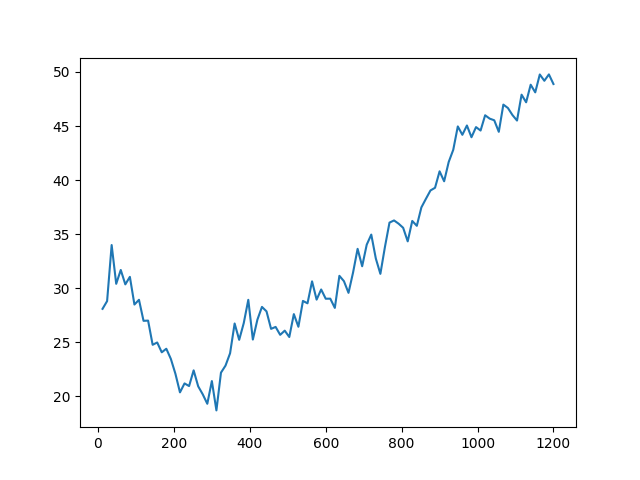
\includegraphics[width=0.85\textwidth]{4}
	\caption{NaiveS的MSE-周期曲线}
\end{figure}
\newpage
从图中可得,$Naive_s$大致在310h处达到最优性能。因此可以判断,该序列的周期大约为310h。
\end{mySol}


\end{document}